\documentclass[12pt,conference]{IEEEtran}
\usepackage[utf8]{inputenc}
\usepackage{amsmath}
\usepackage{amsfonts}
\usepackage{amssymb}
\usepackage{graphicx}
\usepackage[backend=bibtex,sorting=nyt,style=ieee]{biblatex}
\addbibresource{bib/sdn.bib}
\addbibresource{bib/trust.bib}
\author{Christopher C. Lamb \\ Department of Electrical and Computer Engineering \\ The University of New Mexico}
\author{
\IEEEauthorblockN{Christopher C. Lamb}
\IEEEauthorblockA{Dept. of Electrical and Computer Engineering\\
The University of New Mexico\\
Albuquerque, New Mexico 87131\\
Email: cclamb@ece.unm.edu}
\and
\IEEEauthorblockN{Gregory L. Heileman}
\IEEEauthorblockA{Dept. of Electrical and Computer Engineering\\
The University of New Mexico\\
Albuquerque, New Mexico 87131\\
Email: heileman@ece.unm.edu}
}

\title{Towards Robust Trust in Software Defined Networks}
\begin{document}


\maketitle
\begin{abstract}
Software defined networks (SDNs) are becoming more popular in industry, though currently still only deployed by very technically-savvy organizations.  Nevertheless, as the advantages of using SDN become more clear, future adoption promises to be high, with all network equipment vendors quickly moving to deploy products providing SDN capabilities.  This impending wider adoption demands that security implications within SDN be more clearly understood.  Today, mechanisms through which vendors can provide enhanced integrity and availability as well as agent-centric authentication and non-repudiation are poorly understood and have yet to be thoroughly investigated.  In this paper, we present our current work outlining how we can define trust in SDN and what trust in SDN means for various operational components.  We also address what the operational characteristics that impact trust propagation are, and present promising approaches to managing trust within SDN as an extension of these definitions and attributes.
\end{abstract}

\section{Introduction}
Clearly, Software Defined Networks (SDNs) are here to stay. The specific technologies are still in question, in that the community has yet to decide if OpenFlow will be the most common southbound protocol, or if it will be supplanted by some other alternative~\cite{rfc6241}.  Nevertheless, intense industry involvement in SDN technologies and techniques makes it clear that organizations will be adopting SDN in the future, whether they would like to or not~\cite{opendaylight}.  In order to effectively deploy SDN systems, we need to have a clear understanding of how we can secure them.  To begin to secure SDN, we need to establish a more general picture of how trust propagates through SDN systems so we can more clearly envision how we can take advantage of hardened or redundant systems to enhance the security posture of deployed systems.  The way we extend trust to system components in operational systems is key to defining and clarifying overall security postures in SDN architectures.

The contributions of this paper are describing the primary components of oeprational SDN systems, defining the trust relationships that exist and why they are important, outlining why SDN systems differ from other systems with established trust models, and then detailing which approaches to defining SDN trust are most promising and why.

This paper represents our work in progress toward defining a rigorous trust model for SDN systems.  As of today, we have framed the problem and defined a general SDN control architectural model over which we will begin to apply mathematical trust models.  This paper will describe this reference model for the SDN control plane, highlight the key attributes of realistic SDN control planes a trust model must handle, and describe promising approaches to mathematically describing trust in SDN.  We close the paper with references to related work and our future plans in this area.

\section{Trust in SDN}
In order to frame the discussion of trust appropriately, we first propose a common model for the SDN control plane.  This model allows us to define the common elements we need to examine, to describe the trust relationships, and describe precisely why these components are forced to trust other elements in the overall trust model.  Here, we are going to limit our taxonomy to objects and classes based in OpenFlow inspired SDNs.

When modern SDN with OpenFlow was first developed, it consisted of a two layers --- a controller layer sending messages to a programmable switching layer.  This provided separation between the control and data forwarding planes, enabling new capabilities for network innovation.  In this early model, controllers maintained local databases of network state or local context to make packet forwarding decisions.  This model was certainly useful and provided new capabilities previously unable to be deployed.  Systems were able to take advantage of fine-grained system and user authentication and authorization, for example, at lower network levels than previously attempted.  These initial configurations used the OpenFlow protocol to send information between controllers and switches, resulting in a two layer system~\cite{openflow1.0}.

Over time, researchers began to incorporate other external elements, primarily to provide context information with respect to the current network.  These data repositories could provide controllers with much more information about the current state of a given network.  This information would then be used to make routing decisions.  It could furthermore be shared between multiple geographically distributed controllers, providing more global insight into current operational state while empowering local controllers to appropriately optimize their local environments~\cite{HeShMc:12,ScSu:13}.

Shortly thereafter, due to the combined drives to both provide support for multiple protocols for switch management and to enable more established network vendors to claim a more competitive position in the burgeoning SDN market, software engineers began to propose architectures similar to what we see today in OpenDaylight.  These systems began the current trend toward northbound and southbound interface separation, where the southbound interfaces used various protocols to communicate with network forwarding hardware while northbound interfaces enabled applications to submit control preferences, requests, or commands to the overall network management system~\cite{opendaylight,big_network_controller}.

\subsection{A Common Structural Trust Model}
This gives us five distinct elements in a typical modern SDN system, as shown in Figure~\ref{fig:reference-model}.  This includes a {\bf host}, the originator and termination of network traffic.  These are network clients and can include computing devices of any profile, from watches to refrigerators and cars to typical workstations and notebooks.  

\begin{figure}[!t]
\centering
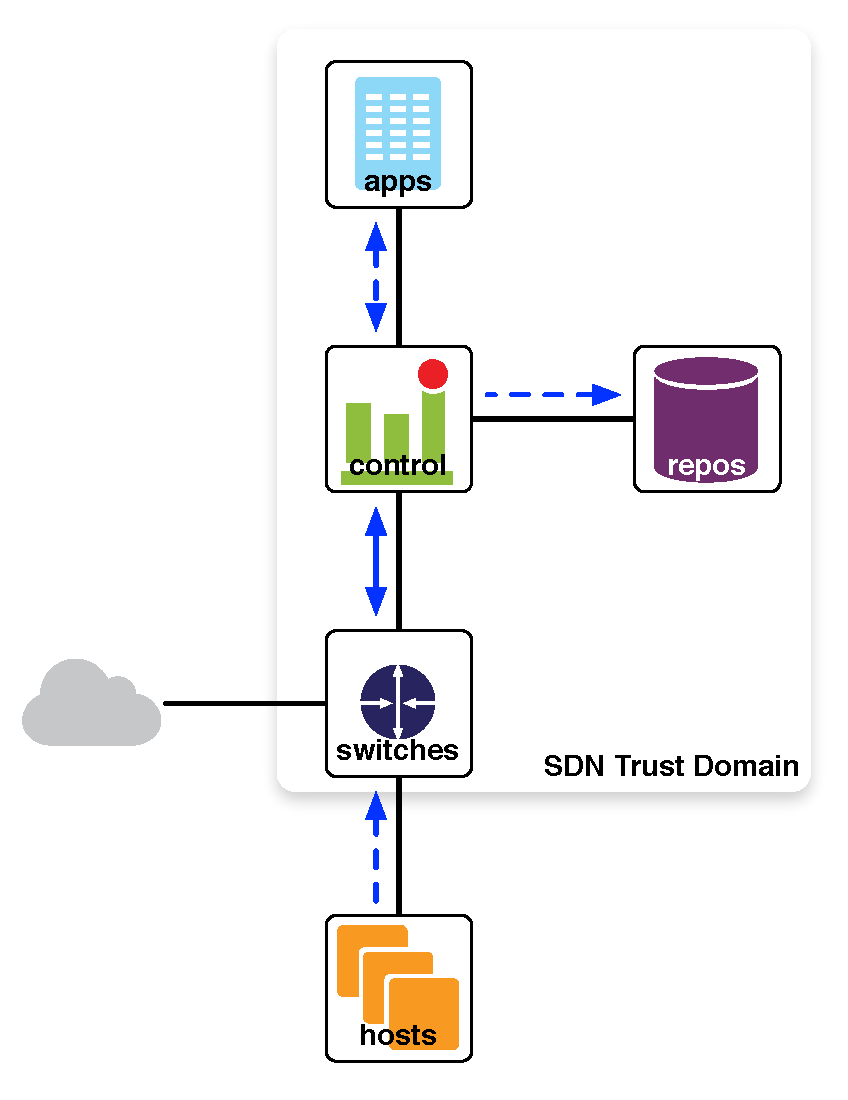
\includegraphics[width=2.5in]{images/reference-model.pdf}
\caption{A reference model for SDN based on modern systems with north- and south-bound interfaces.  Note the contextual data repositories, and the highlighted trust domain specific to SDN.}
\label{fig:reference-model}
\end{figure}

Hosts connect to {\bf switches}, which perform any number of network traffic management including routing.  Switches connect hosts to larger networks and the wider internet.  

In SDN systems, switches are controlled by {\bf controllers}, which implement rules describing what flows should be allowed.  Note that in modern SDNs, all switches need not be SDN switches to enable programmable networks, but within this model we only consider SDN-enabled switches as our focus is on SDN networks and trust, not traditional non-programmable network hardware.  Controllers implement policies and host programs that process both northbound and southbound interfaces to support application and switch communication respectively.  

In order to manage networks effectively and apply defined policies appropriately, controllers need access to wider contextual information including operational state, overarching policy information, authentication data, and the like.  This information is contained in groups of {\bf repositories}, hosted in various geographic locations.  Information contained in repositories can very well be cached, though in the scope of this model we will regard repository caches as repositories as they still provide relevant and necessary information to controllers.  

Finally, we include groups of {\bf applications} that submit network management requests to various controllers.  The controllers can regard such requests as optional or required, depending on the authority of the submitting application.

All communication is over {\bf networks} of various physical types.  These networks can be wireless or wired, using virtually any protocol, though IP networks are arguably the most common realistically and originally the only supported network type~\cite{openflow1.0}.  We can use different physical networks for control plane communication or a single network for both control and data plane packets.

The next sections describe from a confidentiality, integrity, avaibility, non-repudiation, an authentication perspective the types of trust that components expect within a typical SDN.  The hosts and relationships outlined below follow those presented in Figure~\ref{fig:reference-model}.

\subsubsection{host $\leftrightarrow$ switch} A host must be able to trust that a switch will provide flow routing services compliant to local policies.  This may or may not include respecting the confidentiality of the traffic. In some cases, like traffic in places of employment, confidentiality may not realistically be an expectation because of content monitoring or data lost prevention needs.  Integrity expectations with respect to actual traffic are high in all cases.  Certain network middleboxes may change packet header information, but should never alter data bytes within a given packet.  Availability expectations for networks overall are very high as well.  Hosts have no expectation of non-repudiation of switch services as all flow management operations are transient.  Ideally, hosts would be able to authenticate switches however without or with very little {\sl a priori} knowledge.  Also, note that these expectations are in fact of the entire network; the connecting switch is just representative of the network to the host.

Switches do not access services provided by hosts, and need to have very little trust in a given host.  They may however enforce non-repudiation with respect to individual flows or packets and users generating given flows or packets.  A typical example of this kind of requirement stems from network forensics needed after malicious insider activities. Switches may also require host and user authentication.  This kind of authentication is a prerequisite for non-repudiation, but may also be needed in networks with strict policies regarding who can connect.

\subsubsection{switch $\leftrightarrow$ controller}
Switches extend a tremendous amount of trust in controllers.  Some of that trust is in fact transitive as well, based on trust extended first to switches by attached hosts.

\subsubsection{controller $\leftrightarrow$ repository}

\subsubsection{controller $\leftrightarrow$ application}

\subsection{Differentiating Attributes of Software Defined Networks}

\subsection{Promising Approaches to Trust Management}

\section{Related Work}

\section{Conclusions}

\printbibliography
\end{document}